\documentclass[11pt,a4paper]{article}
\usepackage[T1]{fontenc}
\usepackage[left=3cm, right=3cm, top=3cm, bottom=3cm]{geometry}
\usepackage{graphicx}
\usepackage{mathtools}
\usepackage{amssymb}
\usepackage{amsthm}
\usepackage{thmtools}
\usepackage{nameref}
\usepackage{hyperref}
\usepackage{times}
\begin{document}
\begin{center}
		\Large \textbf{Flat Field Generation from observations.}\\
		\normalsize Janmejoy Sarkar
\end{center}
	The system wide flat field of SUIT is necessary to remove large scale patterns seen in the SUIT images. These patterns 	arise due to optical or electronic reasons. The off pointed solar images are combined as per the method described above and we get the illumination as in Figure \ref{fig:flat_field}. 
	
	Our motivation is to select size scales that affect our observations. In this case, it is a diagonal series of lines repeating at intervals of 310 pixels across the direction perpendicular to the lines. A test is performed to confirm the methodology and the procedure used to isolate the striped nature of the uneven illumination.
	
	\section{Methodology}
	\begin{itemize}
		\item Aditya is moved on roll and pitch axes in steps of 8 arc mins. The entire field of view (FOV) is covered by the solar disk with 28 pointings of the satellite.
		\item The observations are made with 11 filter combinations of SUIT over a period of 18 days (Figure \ref{fig:off pointing}).
		\item Scattered light and bias is removed from each image before processing them to generate the flat field.
		\item The images are sorted and any partial frames are discarded.
		\item On an average, approximately 14 images are obtained per filter, per pointing of SUIT.
		\item The scatter and bias corrected images are added to increase the signal to noise ratio (SNR) of the raw data. We shall call these \textit{Summation Images.}
		\item The \textit{Summation Images} are combined using the developed algorithm to create the illumination pattern. We shall call this \textit{Blended Image}.
		\item The feature scale of interest is identified. in our case, the periodic stripe like pattern is seen to repeat itself after every 620 pixels along the direction perpendicular to the stripes.
		\item We apply a boxcar blurring to remove all structures smaller than 6.5 px in size. This is necessary to get rid of the small scale fluctuations in the image due to pixel response non uniformity or small contaminants on the CCD. We shall call this \textit{Small Scale Removed Image}.
		\item A copy of the blurred image is generated. Boxcar blurring of kernel size 620 px is applied on this copy to derive the large scale non uniformity of illumination in the image. This could be arising from non uniform ilumination of the CCD due to the telescope optics, or due to limb darkening of the sun around the edges of the image. We shall call this \textit{Large Scale Illumination Profile}.
		\item The bluring kernel size of 620 pixels is derived analytically based on the frequency of the stripes appearing on the image. The methodology used for this is described ahead in the document.
		\item The \textit{Large Scale Illumination Profile} is divided from the \textit{Small Scale Removed Image} to extract the feature of our choice, the stripe like pattern (Figure \ref{fig:flat_field}).
	\end{itemize}
	
	\subsection{Simulation to validate blurring kernel size}
	\begin{itemize}
		\item A stripe like pattern is generated using a sine function across the different rows of a 4096x4096 grid to mimic the stripe like pattern in \textit{Summation Image}.
		\item Provision is kept to vary the size and frequency pattern of the stripe.
		\item Artificial dust spot, poission noise, 1\% PRNU, and read noise with RMS error of 8 photo electrons is added to the image to mimic real observation generated from SUIT.
		\item The \textit{Large Scale Illumination Profile} is generated using the above steps, and the percentage standard deviation of the same is measured within a 2596x2596 px area at the center of the image.
		\item The standard deviation of the \textit{Large Scale Illumination Profile} will be influenced by large scale features, as all small scale structures are removed from it.
		\item The \textit{Large Scale Illumination Profile} will be devoid of any residual of the stripe like pattern provided, the blurring kernel size matches the thickness of the stripes. Mismatch of the kernel size would leave a residual of the stripe like pattern, causing an increase in percentage standard deviation.
		\item The percentage standard deviation is plotted with kernel sizes (Figure \ref{fig:optimal}) and it is seen that it is the lowest at kernel sizes comparable to the wavelegth of the sine function used to generate the striped pattern.
		\item This is repeated for various wavelengths of the sine function and in every case the comparable kernel size showd the least residual in the \textit{Large Scale Illumination Profile} .
	\end{itemize}
	
	\begin{figure}
		\centering
		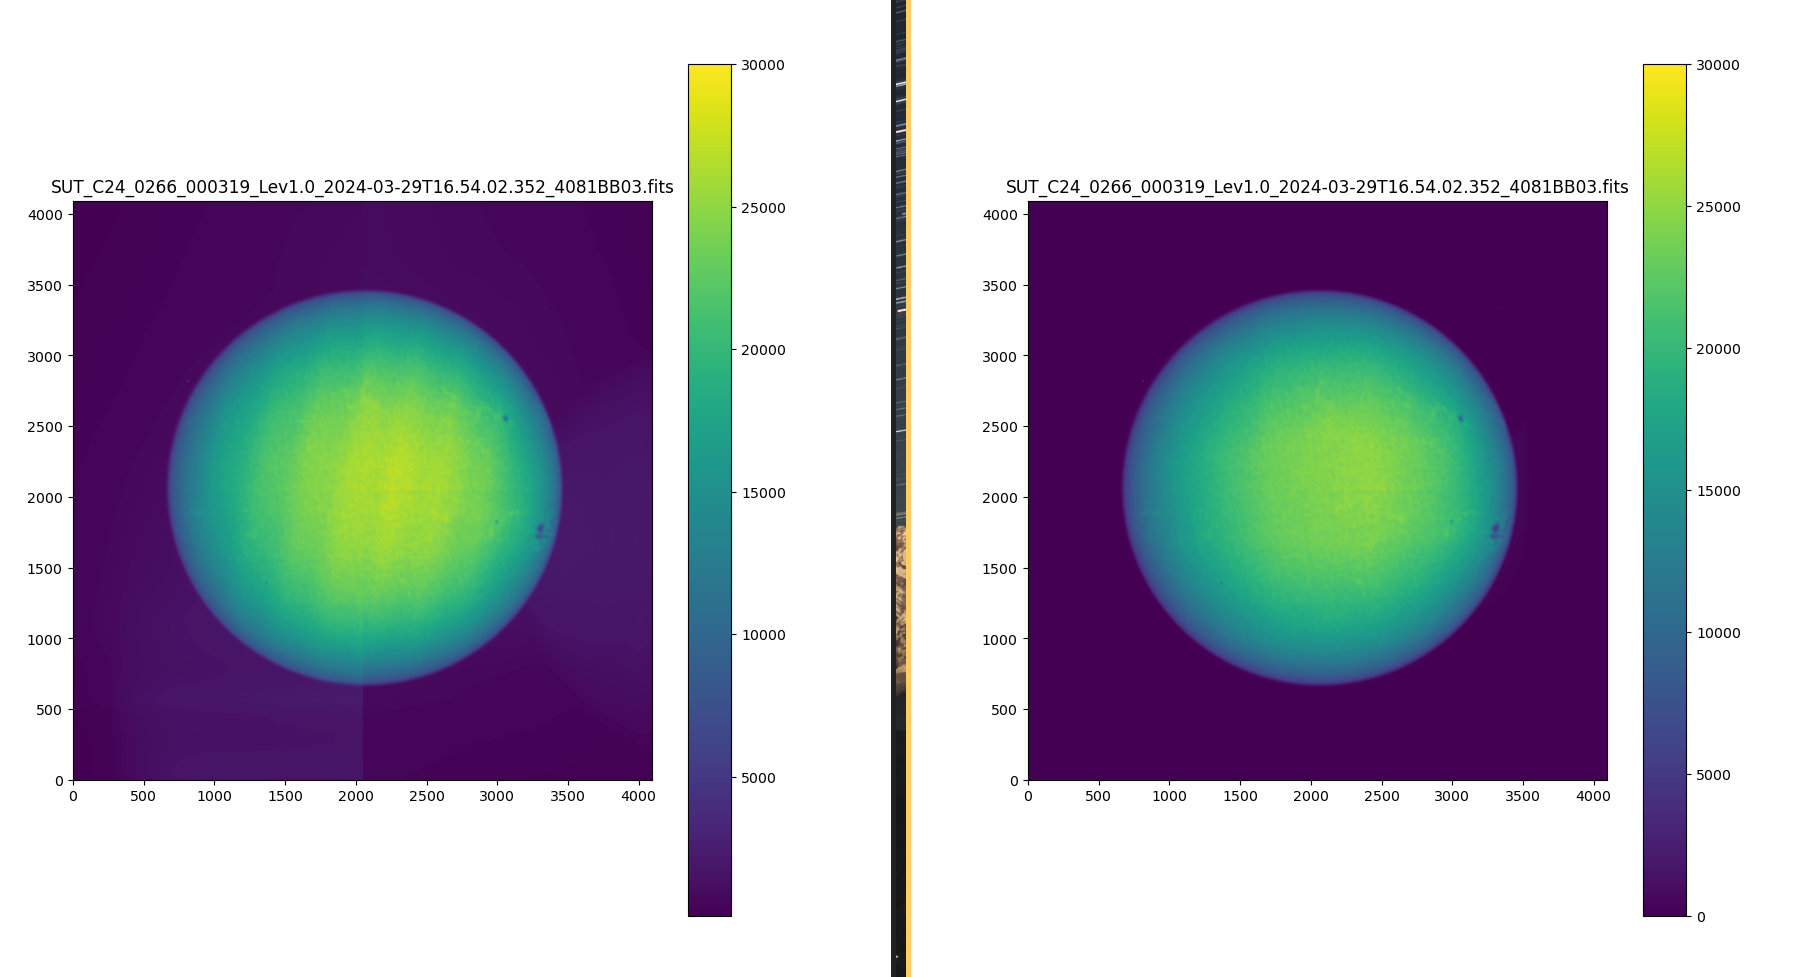
\includegraphics[width=0.7\linewidth]{pics/screenshot_2024-06-06_12-24-27}
		\caption{SUIT Image, before and after flat field correction}
		\label{fig:compare}
	\end{figure}
	
	\begin{figure}
		\centering
		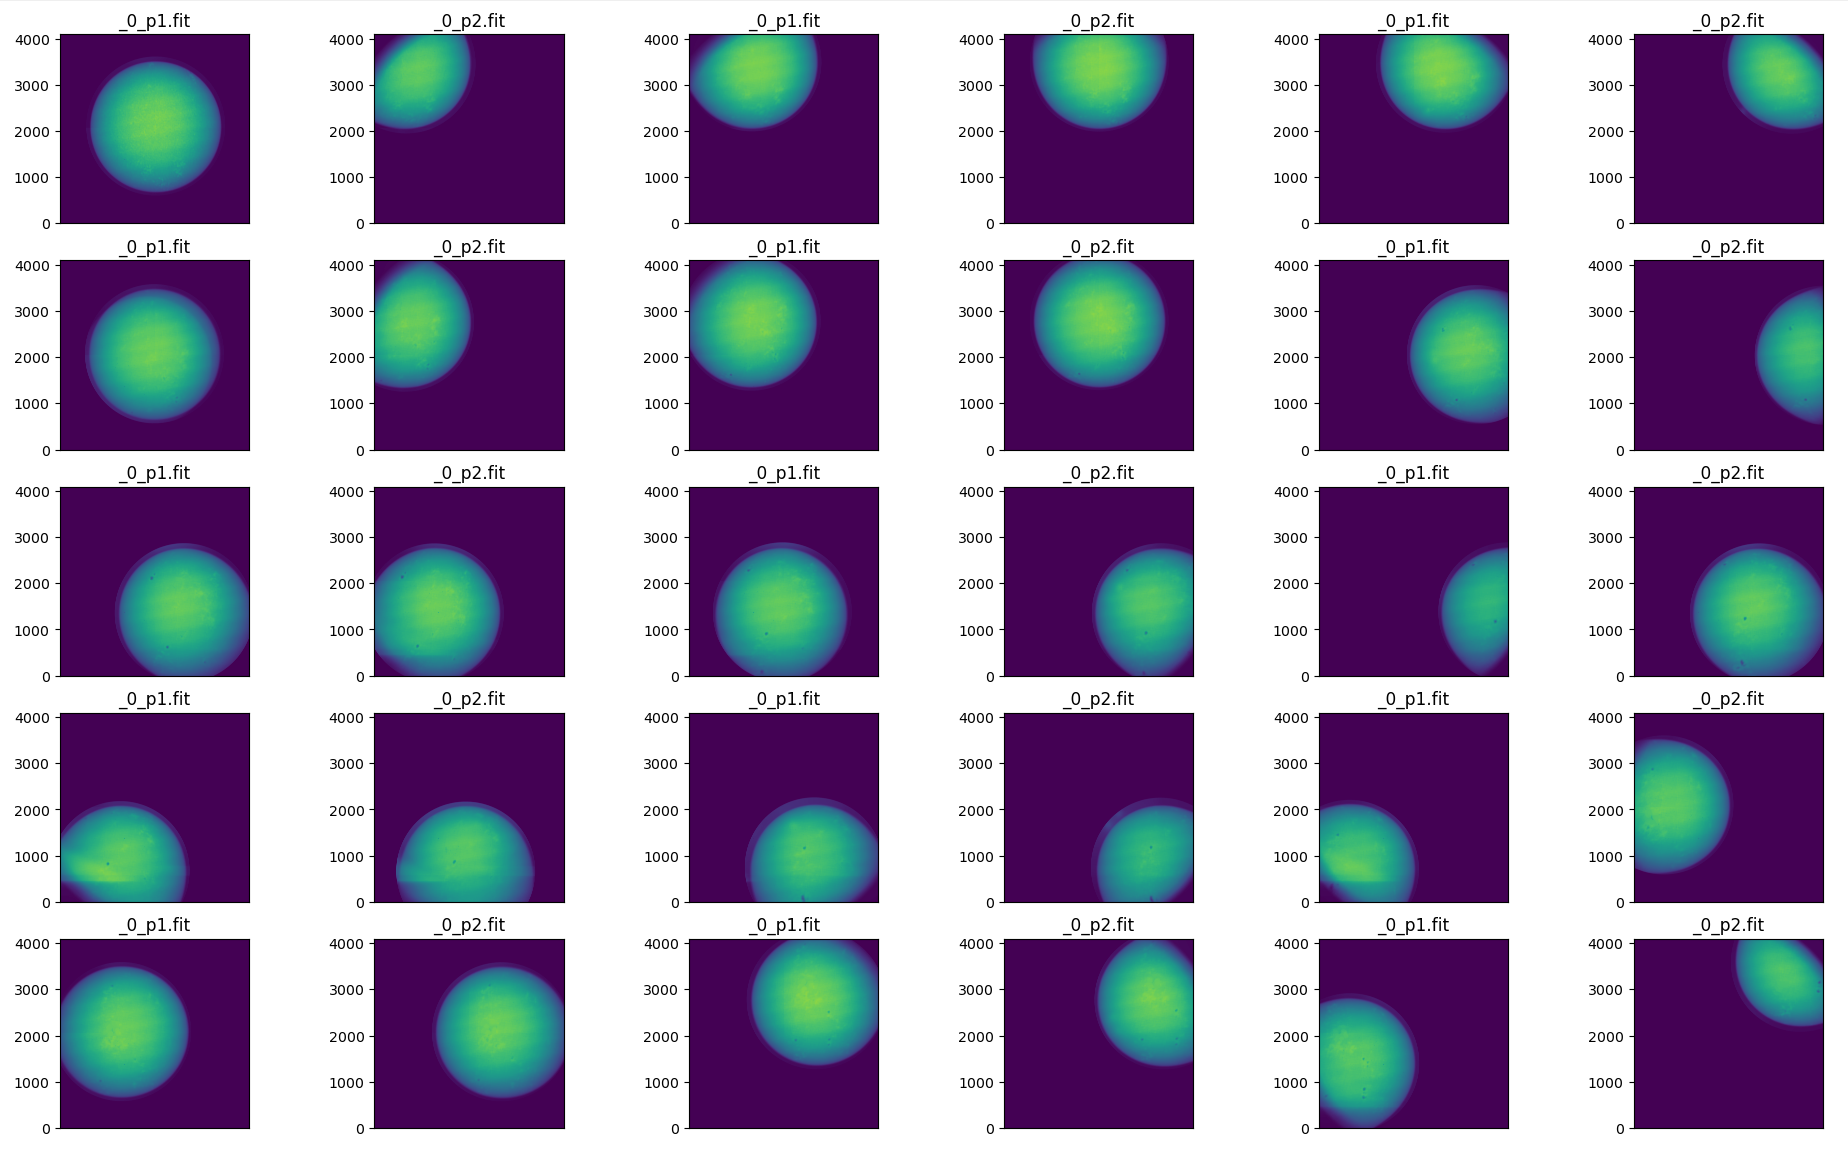
\includegraphics[width=0.7\linewidth]{pics/screenshot_2024-06-06_11-35-10.png}
		\caption{Solar off pointing- NB06 images.}
		\label{fig:off pointing}
	\end{figure}
	
	\begin{figure}
		\centering
		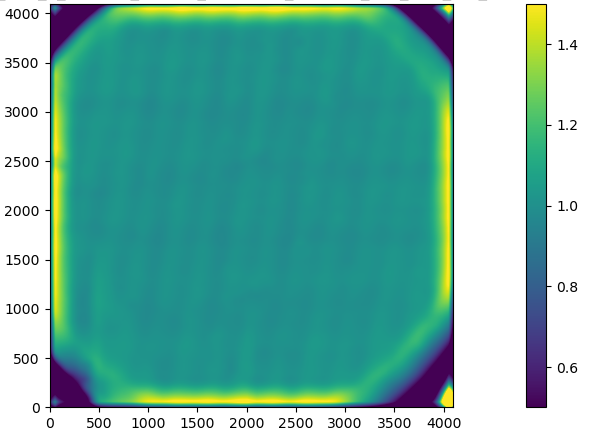
\includegraphics[width=0.5\linewidth]{pics/screenshot_2024-06-17_12-30-11.png}
		\caption{Flat field image}
		\label{fig:flat_field}
	\end{figure}
	
	\begin{figure}
		\centering
		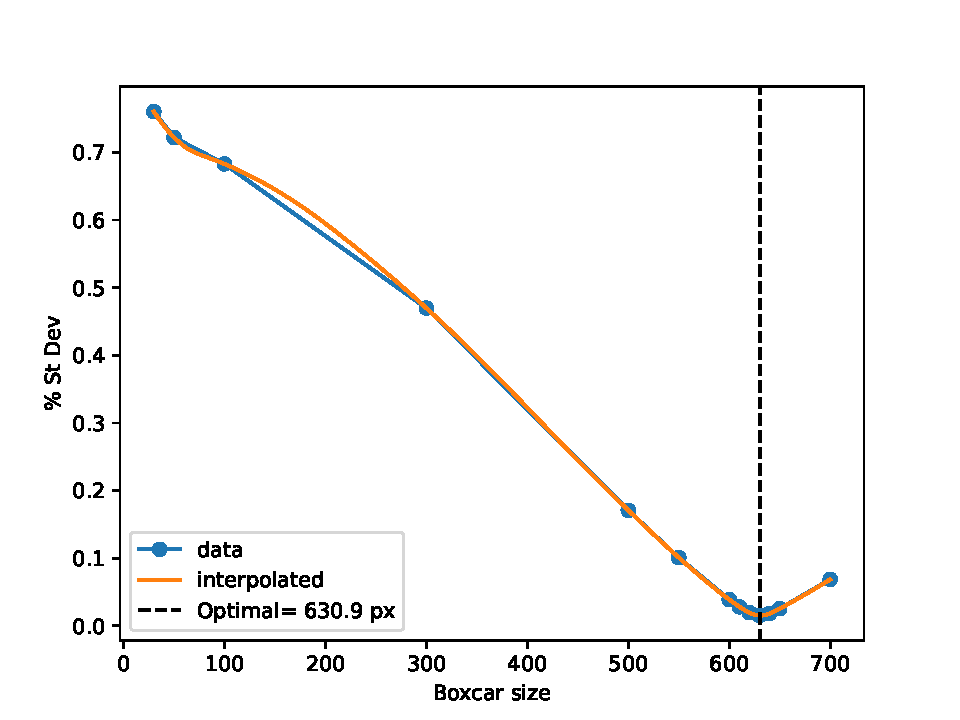
\includegraphics[width=0.7\linewidth]{pics/13.pdf}
		\caption{Optimal blurring kernel size for stripe pattern repeating every 630.2 px. The standard deviation of the  \textit{Large Scale Illumination Profile} is minimum for this blur size.}
		\label{fig:optimal}
	\end{figure}
	
	\subsection{Flat Field Validation}
		The flat field is generated from real SUIT observations and applied on SUIT LED images. Optimized kernel sizes are used to generate the SUIT flat field to remove the stripes seen in the image.
	\begin{itemize}
		\item A stack of 20 LED images with similar illumination pattern is used as the raw image. A stacked image is used to increase the SNR and reduce poission noise.
		\item The LED image is divided by the flat field to create the corrected image.
		\item A cut across the image is taken such that the striped pattern is registered, while ensuring the LED illumination pattern is approximately constant across the line.
		\item Line profile before and after the flat field correction reveals that the periodic rise and fall in brightness has been corrected by the flat field. This is seen in both LED wavelengths of 355 nm and 255 nm (Figure \ref{fig:validation}).
		\item A  box of $20 \times 20$ px is chosen from a dark and a bright stripe on the images lying on the marked line. The mean value within the two boxes are calculated. The difference of the mean values is divided by the total mean count of the two boxes put together to find the percentage variation in intensity between the dark and bright patch.
		\item It is seen that the variation in intensity between the two patches are 0.54\% before flat field correction, which improved to 0.11\% after correction, as seen in 255 nm LED image.
		\item The variation in intensity between the two patches are 1.44\% before flat field correction, which improved to 0.03\% after correction, as seen in 355 nm LED image.
		\item Further optimization is ongoing to improve the quality of flat fielding by isolating structures from the images and correcting them in with a multiscale approach.
	\end{itemize}
	
	\begin{figure}
		\centering
		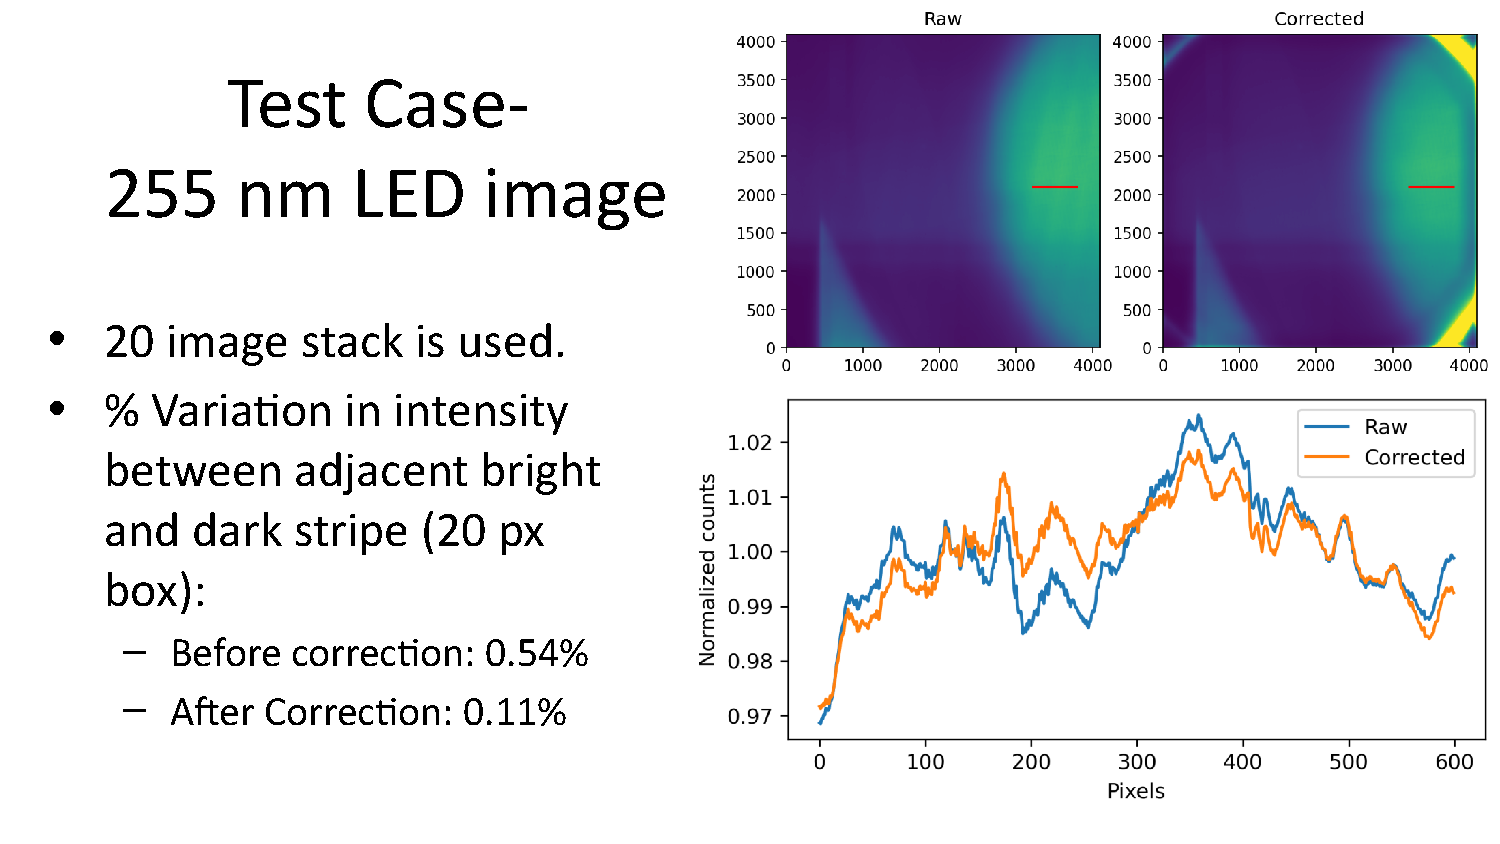
\includegraphics[width=0.9\linewidth]{pics/12.pdf}
		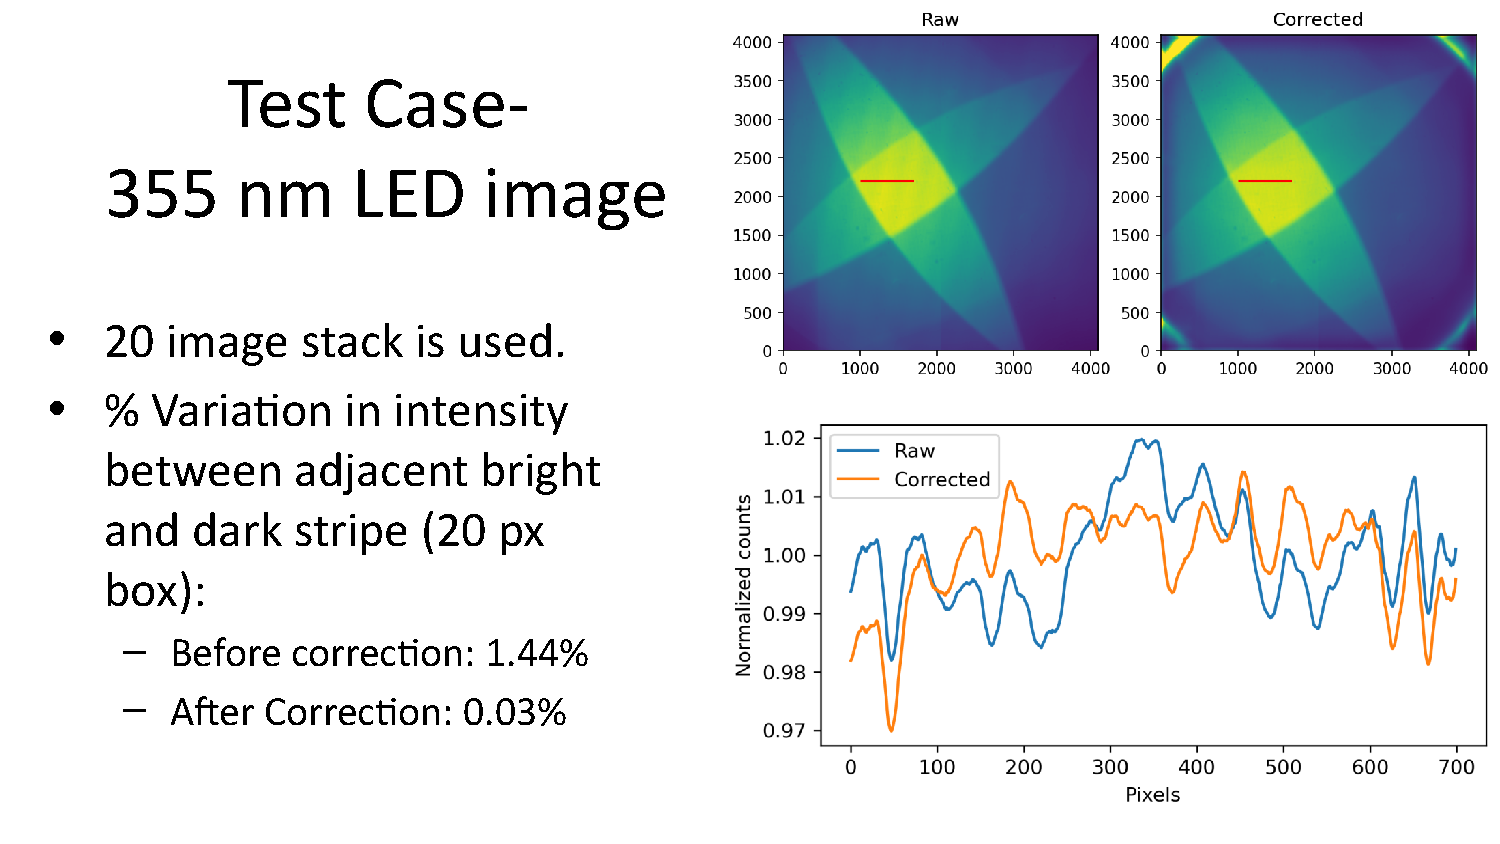
\includegraphics[width=0.9\linewidth]{pics/11.pdf}
		\caption{Flat Field validation with 355 nm and 255 nm LED images respectively.}
		\label{fig:validation}
	\end{figure}
	
\end{document}